\documentclass{article}
\usepackage[margin=1in]{geometry}
\usepackage[utf8]{inputenc}
\usepackage{mathtools}
\usepackage{enumitem}
\usepackage{fancyhdr}
\usepackage{chngcntr}
\usepackage{tikz}

\lhead{Evan Kohilas - z5114986}
\rhead{COMP3821 - Assignment 4}
\pagestyle{fancy}
\title{A17S1N4}
\counterwithin*{equation}{section}
\usepackage{parskip}
\begin{document}

\begin{center}
    \begin{LARGE}
        COMP3121\\
        Assignment 4\\
        A17S1N3\\
        \hrulefill\\
        Evangelos Kohilas\\
        z5114986\\
        \hrulefill
    \end{LARGE}

    \begin{large}
        By submitting this document you are confirming that all the answers are your work and are not take from any other sources unless clearly mentioned.
    \end{large}

\end{center}

\section*{Question 1}
sort either the weights or the IQs in decreasing order, then we can find the longest subsequence of the unsorted list.

For each element from i to n in the list, we find a subseqence from 1 to i of which the values are strictly increasing and the subseqeunce ends with Ai
we do this recursivly, where for each a[m] such that m < i and a[m] < a[i], picking the maximum value, and then enxtending it with a[i].

\textbf{Proof of optimality:}\\
This soultion is optimal as if we truncate the solution we still produce an optimal solution for the subproblem P(m)


\begin{verbatim}
code goes here
\end{verbatim}

\pagebreak
\section*{Question 2}
divide up the wood into the n total peices that will be cut
m(i, j) for all
then for every i < n - 1, calculate the minimum value of (A[i] + A[i+1]) + (A
min cost = min( A[0]+A[i] + A[i+1]A[n]:  1 < i < n - 2)
min cost = min( m(0,i) + m(i+1, n):  1 < i < n - 2)
m(i, j)  = min( m(i,k) + m(k+1, j): i <= k <= j - 2

\textbf{Proof of optimality:}\\
text

\section*{Question 3}
for every

\textbf{Proof of optimality:}\\
let $S = \{p_1, p_2, p_3, \ldots, p_n\}$\\
let $O$ be the set of the optimal solution.\\
let $S_i$ be the subset of $S$ after $i$ iterations where $0 \leq i \leq n$.

We prove by induction that $O$ will always be a subset of $S_i$.

When $i = 0$, no people have been removed, and so $O$ remains a subset of $S_0$

Assume $i = k$ such that after $k$ iterations, $O$ is a subset of $S_k$

let $i = k + 1$:\\
$O$ will still remain as a subset of $S_{k+1}$ as $p_{k+1}$ will only be removed if $p_{k+1}$ doesn't satisfy the two constraints.

Therefore by induction, since $O$ is still a subset of $S$, $S$ is optimal since $|S| \geq |O|$, as we are trying to maximise the number of invitees.

\section*{Question 4}
\begin{enumerate}[label=\alph*)]
    \item
    Given the following arrangement,
    \begin{center}
    
\begin{tikzpicture}
        \tikzset{circles/.style={draw, circle, very thick, minimum size=5mm}}
        \node [circles, fill=black] (1) at (0, 0){};
        \node [circles, fill=black] (2) at (2, 0){};
        \node [circles]             (3) at (4, 0){};
        \node [circles]             (4) at (6, 0){};
        \node [circles, fill=black] (5) at (8, 0){};
        \node [circles]             (6) at (10,0){};
    \end{tikzpicture}
    \end{center}

    By using the closest pair method (the proposed algorithm) our total length will be $5 + 1 + 1 = 7$
    \begin{center}
    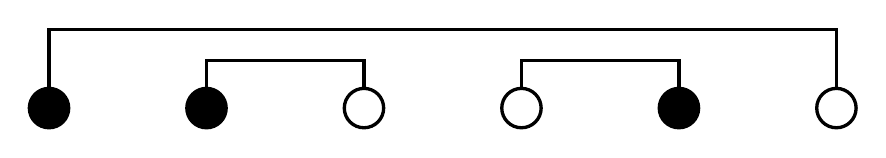
\begin{tikzpicture}
        \tikzset{circles/.style={draw, circle, very thick, minimum size=5mm}}
        \node [circles, fill=black] (1) at (0, 0){};
        \node [circles, fill=black] (2) at (2, 0){};
        \node [circles]             (3) at (4, 0){};
        \node [circles]             (4) at (6, 0){};
        \node [circles, fill=black] (5) at (8, 0){};
        \node [circles]             (6) at (10,0){};
        \draw [very thick] (1) |- +(0,  1) -| (6);
        \draw [very thick] (2) |- +(0,0.6) -| (3);
        \draw [very thick] (4) |- +(0,0.6) -| (5);
    \end{tikzpicture}
    \end{center}

    This is not optimal as the following solution has a shorter length of size $2 + 2 + 1 = 5$
    \begin{center}
    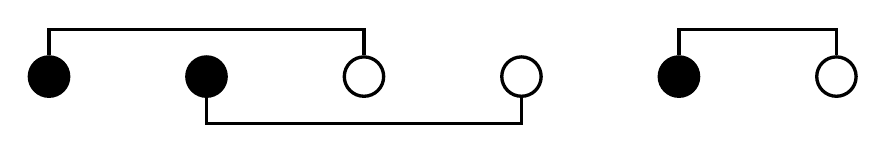
\begin{tikzpicture}
        \tikzset{circles/.style={draw, circle, very thick, minimum size=5mm}}
        \node [circles, fill=black] (1) at (0, 0){};
        \node [circles, fill=black] (2) at (2, 0){};
        \node [circles]             (3) at (4, 0){};
        \node [circles]             (4) at (6, 0){};
        \node [circles, fill=black] (5) at (8, 0){};
        \node [circles]             (6) at (10,0){};
        \draw [very thick] (1) |- +(0, 0.6) -| (3);
        \draw [very thick] (2) |- +(0,-0.6) -| (4);
        \draw [very thick] (5) |- +(0, 0.6) -| (6);
    \end{tikzpicture}
    \end{center}

    \item
        Going from left to right, we can produce an optimal solution by matching each dot with its earliest possible match.

        \textbf{Proof of optimality:}\\
        Let $A$ be our greedy solution produced by our algorithm and $O$ be the optimal solution.

        If we violate our greedy algorithm, then there are two cases that can occur.

        If we swap two pairs in $A$ such that a pair finishes in the position of an earlier pair, then the earlier pair will finish in the position of the later pair, but the total length will not increase as both will have changed by the same amount.

        If we swap two pairs in $A$ such that a pair finishes in the position of a later pair, then the length of that pair will increase, but the length of the later pair will either decrease by an equal amount such that the total length will not increase, or not decrease, such that the total length has increased.

        Therefore $A$ is optimal as $O$ does not offer a better solution than the one produced by $A$.

\end{enumerate}

\section*{Question 5}
To complete $n$ tasks with as low total penalty as possible, we pick the highest penalty task and schedule it to be completed as late as possible before incurring a penalty. If the picked task is scheduled to be completed in such a way that would incur a penalty, we ignore it, scheduling it to be completed after all tasks without penalty have been completed. We repeat this until all tasks have been scheduled.

\textbf{Proof of optimality:}\\
Let $A$ be our greedy solution produced by our algorithm and $O$ be the optimal solution.

We can violate our greedy algorithm by swapping tasks from $A$ to $O$, such that they are either scheduled earlier, or scheduled later.

In both cases, by doing so we have either:
\begin{enumerate}
    \item Scheduled the tasks such that there is no change to the total penalty.
    \item Scheduled one of the tasks to be past its due date, and thus increasing our penalty.
    \item Scheduled a lower cost task to be before its due date, but scheduled a higher cost task after its due date, thus increasing out total penalty.
\end{enumerate}

Therefore $A$ is optimal as all cases cannot create a better solution than the greedy one produced by our algorithm.

\section*{Question 6}
To calculate the first 10 books that we need to borrow, we iterate through the sequence of books, adding each book to a set and continuing until our set is of length 10. Whenever we come across a book we need that is not in our set, we make another trip to the library, creating a new set and iterating as before.

\textbf{Proof of optimality:}\\
let $B$ be the sequence of books.\\
let $A$ be the set of the first 10 unique books from $B$ to keep produced by our algorithm.

Suppose $A$ is not optimal, and assume $O$ be the optimal solution.\\
If we violate the greedy algorithm, taking one less book, then $|O| = 9$.

If $|O| = 9$ then one of two things have occurred:

Either we have moved a book to the next set such as the next set will contain the $20^{th}$ book that we will need, as it will be the same as the book removed.

Or we have removed a book such that we require an additional trip to compensate for the $20^{th}$ book that could not be added to our set.

Therefore, $A$ is optimal as we cannot create a better solution than the greedy one produced by our algorithm.

\end{document}
